\subsection{Pengujian SLAM}
\label{subsec:slamtesting}

\begin{figure} [ht]
  \centering
  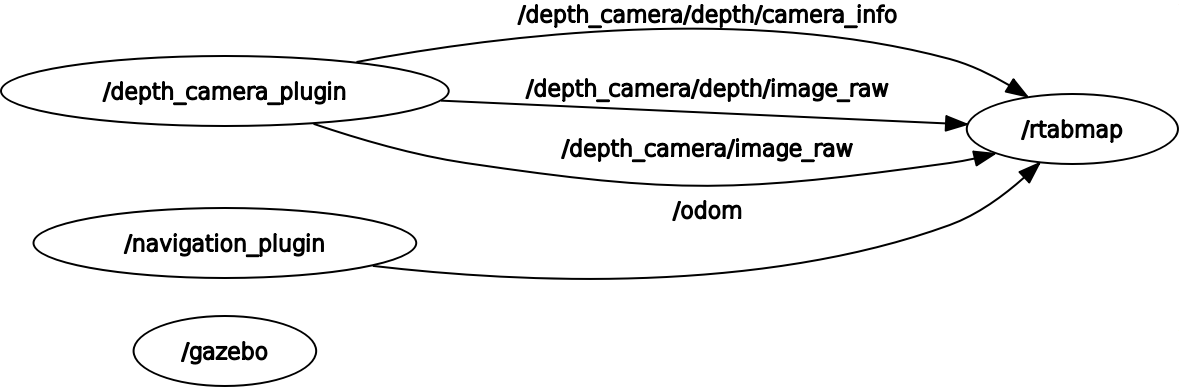
\includegraphics[width=0.45\textwidth]{figures/rosgraph/slam.png}
  \IfLanguageName{english}{
    \caption{Node scheme of the SLAM testing.}
  }{
    \caption{Skema \emph{node} dari pengujian SLAM.}
  }
  \label{fig:rosgraphslam}
\end{figure}


Pengujian SLAM (\emph{simultaneous localization and mapping}) dilakukan di simulasi dengan tujuan untuk menguji kemampuan ruangan virtual dalam mensimulasikan ruangan \emph{real}.
Pada pengujian ini,
  model robot akan bergerak mengelilingi ruangan sambil melakukan pemetaan menggunakan metode SLAM.
Seperti yang terlihat pada gambar \ref{fig:rosgraphslam},
  \emph{node} \lstinline{rtabmap} akan terhubung dengan \emph{node} \lstinline{depth_camera_plugin} dan \emph{node} \lstinline{navigation_plugin} yang akan mengirimkan data citra warna, citra kedalaman, serta odometri yang akan digunakan dalam proses pemetaan ruangan.

\begin{figure} [ht]
  \centering
  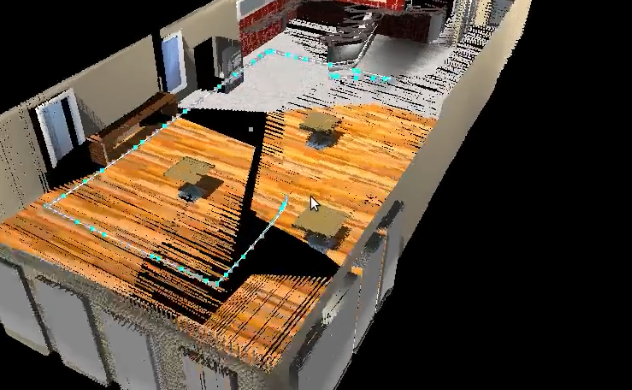
\includegraphics[width=0.4\textwidth]{figures/slam.png}
  \IfLanguageName{english}{
    \caption{Room mapping results.}
  }{
    \caption{Hasil pemetaan ruangan.}
  }
  \label{fig:slam}
\end{figure}


Hasilnya,
  seperti yang terlihat pada gambar \ref{fig:slam},
  proses pemetaan ruangan menghasilkan peta tiga dimensi yang tersusun atas \emph{point cloud} yang membentuk ruangan yang diujikan di simulasi.
Peta tersebut ditampilkan pada GUI yang dimiliki oleh \emph{node} \lstinline{rtabmap}.
Selain itu,
  pada peta tersebut juga tampak visualisasi dari lintasan yang telah dilalui robot sebagai garis dengan titik berwarna biru.
